\section{Ape 1}

\subsection{Vrai ou Faux}
Rappel : Un graphe simple est un graphe
\begin{itemize}
\item sans arêtes multiples
\item sans boucles
 \end{itemize}
\begin{enumerate}
	\item{L'élimination d'un sommet de degré maximum peut augmenter le degré moyen d'un graphe.}
	\item{Un graphe qui ne contient pas de triangle est pibarti}
	\item{Deux graphes qui possèdent un même nombre de sommets et dont les listes de degrés sont identiques sont isomorphes. Même question, si, en plus, les graphes sont connexes.}
	\item{Un graphe simple de 2 sommets au moins possède toujours 2 sommets de degré identiques}
	\item{$\exists$ un graphe simple dont les degrés des sommets sont $\{1,2,2,3,3,4\}$}
	\item{$\exists$ un graphe simple dont les degrés des sommets sont $\{1,1,1,2,3,4,6\}$}	
\end{enumerate}

\begin{solution}
\begin{enumerate}
\item{
$d_{moyen} = \frac{\sum_{1}^{n} d_{i}}{n} \qquad d_{1} \leq d_{2} \leq ... \leq d_{n}$\\
Si on retire $d_{n}$ :
$d_{moyen} = \frac{1}{n-1}  (\sum_{1}^{n} d_{i} -2d_{n}) \qquad \stackrel{?}{>} \qquad \frac{\sum_{1}^{n}  d_{i}}{n}$\\
$\sum_{1}^{n} d_{i} - 2d_{n} \qquad > \qquad \frac{n-1}{n} \sum_{1}{n} d_{i}$\\
$\sum_{1}^{n} d_{i}(1- \frac{n-1}{n}) \qquad > \qquad 2d_{n}$\\
$\implies \qquad \sum_{1}^{n} d_{i} \qquad > \qquad 2n d_{max}$ Impossible !\\
Faux
}
\item{Faux, il peut avoir un cycle de longueur impair $\neq3$ (par exemple 5)}
\item{Faux :\\  
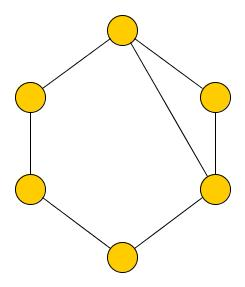
\includegraphics[scale=0.3]{graph_ape1_ex1_3_1}
$ \stackrel{Isomorphe}{\nRightarrow}$
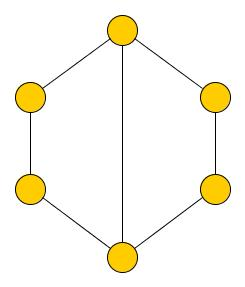
\includegraphics[scale=0.3]{graph_ape1_ex1_3_2}
}
\item{Vrai}
\item{Faux - \textit{Théorème poignée de main} - La somme des degrés est impaire}
\item{Faux, le nœud de degré 6 est relié à tous les autres, donc le nœud de degré 4 et celui de degré 1 ne peuvent pas exister dans ce graphe.}
\end{enumerate}
\end{solution}

\subsection{Démontrez}
\begin{enumerate}
\item{D'un sommet de degré impair, $\exists$ toujours un chemin jusqu'à un autre sommet de degré impair.}
\item{Pour un graph simple et connexe de n sommets, on a $(n-1) \leq |E| \leq \frac{n \times (n-1)}{2}$}
\item{Un graphe simple qui possède plus de $\frac{(n-1) \times (n-2)}{2}$ arêtes est connexe.}
\item{Tout graphe qui possède n sommets et h arêtes possède au moins $n-k$ composantes connexes}
\end{enumerate}

\subsection{Graphe de l'hypercube}
Soit $G_{i}$ le graphe dont les sommets sont des k-tuples de 0 et 1. Deux sommets de G sont adjacents si leurs k-tuples ne diffèrent qu'en une seule position. Montrez que le graphe est biparti, k-régulier et donnez son nombre arrêtes.

\subsection{Parcours fermés}
Formule : $(n-1)^{k} + (n-1)(-1)^{k}$
\begin{enumerate}
\item{Comptez le nombre de parcours fermés de longueur k dans $K_{n}$}
\item{Comptez le nombre de parcours fermés de longueur k dans $K_{k,n}$}
\end{enumerate}

\subsection{Trouvez le nombre de parcours de longueur k du sommet A à lui-même.}
\begin{figure}
\center
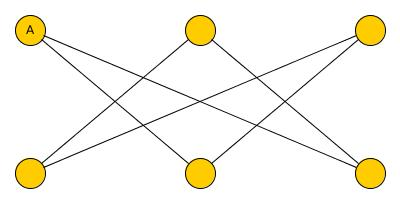
\includegraphics[scale=0.5]{graph_ape1_ex5}
\end{figure}

\subsection{Démonstration - Les rois du graphe}
Un tournoi de n joueurs est un graphe complet $K_{n}$ dans lequel on a choisi une direction pour chaque arête. $\exists$ une arête $(u,v)$ lorsque u a remporté sa partie contre v. Un sommet u d'un tournoi est un roi si quel que soit le sommet v du graphe, il y a une arête $(u,v)$ où il a une arête intermédiaire w et des arêtes $(u,w)$ et $(w,v)$.

Prouvez qu'il existe toujours au moins un roi.
Utiliser ce résultat pour montrer que dans le cas où aucun sommet n'a un degré entrant nul, il y a toujours au moins 2 rois.


